%*********************************************************************
% gdutthesis: 广东工业大学论文模板
% 2021/11/09 v0.1c
%
% 重要提示:
%   1. 请确保使用 UTF-8 编码保存
%   2. 请使用 XeLaTeX 或 LuaLaTeX 编译
%   3. 请仔细阅读用户文档和 Wiki
%   4. 修改、使用、发布本文档请务必遵循 LaTeX Project Public License
%   5. 不需要的注释可以尽情删除
%*********************************************************************
\documentclass[
  % type=doctor
  type=master
  % type=promaster
]{gdutthesis}

% 宏包在这里加载
\usepackage{siunitx}[=v2]
\usepackage{zhlipsum,lipsum}

\gdutsetup{
  style = {
    cover           = {true},
    % cover           = {false},
    % font            = {garamond},
    % font            = {libertinus},
    % font            = {lm},
    % font            = {palatino},
    font            = {times},
    % font            = {times*},
    cjk-font        = {fandol},
    % cjk-font        = {founder},
    % cjk-font        = {mac},
    % cjk-font        = {sourcehan},
    % cjk-font        = {noto},
    % cjk-font        = {windows},
    % cjk-font        = {none},
    bib-backend     = {bibtex},
    % bib-backend     = {biblatex},
    bib-resource    = {gdutthesis-template.bib},
    bib-style       = {numerical},
    % bib-style       = {author-year},
    fullwidth-stop  = {mapping},
    % fullwidth-stop  = {catcode},
    % fullwidth-stop  = {false},
    hyperlink       = {color},
    % hyperlink       = {border},
    % hyperlink       = {none},
    hyperlink-color = {default},
    % hyperlink-color = {autumn},
    % hyperlink-color = {business},
    % hyperlink-color = {classic},
    % hyperlink-color = {elegant},
    % hyperlink-color = {fantasy},
    % hyperlink-color = {material},
    % hyperlink-color = {science},
    % hyperlink-color = {summer},
    % hyperlink-color = {graylevel},
    % hyperlink-color = {prl},
  },
  info = {
    title           = {模板射流电解加工微沟槽关键技术研究},
    title*          = {Investigation on masked jet electrochemical machining of micro grooves},
    date            = {2020/5/25},
    author          = {张三},
    author*         = {Zhang San},
    supervisor      = {李四\qquad 教授},
    supervisor*     = {Prof. Li Si},
    supervisor-two  = {王五\qquad 教授},
    supervisor-two* = {Prof. Wang Wu},
    department      = {自动化学院},
    department*     = {Automation},
    major           = {电子信息},
    student-id      = {2112101234},
    chairman        = {赵六\qquad 教授},
    degree          = {工程硕士},
    degree*         = {Master of Engineering},
    keywords        = {电解加工, 微沟槽, 模板, 射流},
    keywords*       = {electrochemical machining, micro grooves, mask, jet},
    secret-level    = {none},
  }
}


\begin{document}

\begin{abstract}
  \zhlipsum[1-4]
\end{abstract}

\begin{abstract*}
  \lipsum[1-4]
\end{abstract*}

\begin{notation}
  $E$ & 能量 \\
  $F$ & 推力
\end{notation}

\gduttableofcontents

\mainmatter

\gdutchapter{绪论}{Introduction}

\gdutsection{本课题研究背景及研究意义}{Background and significance of research}
随着科学技术的进步,产品逐渐向精密化和高性能化发展,具有毫米及微米尺度
微沟槽结构的金属零部件在国防军事、航空航天、新能源、新材料、生物医学、半导
体器件等领域的高技术产品中扮演的角色愈加重要。

\gdutsection{微沟槽电解加工国内外相关研究现状}{Analysis of the research status at home and abroad}
\gdutsubsection{成型电极电解加工}{Shaped cathode electrochemical machining}
采用与微沟槽结构形状对应的成型阴极,例如薄板阴极,片状阴极等,进行微沟
槽电解加工,其特点是方便一次成型微沟槽形状。南京航空航天大学吕焱明等进行了
大长宽比深窄槽电解加工阴极设计以及工艺试验研究\cite{chendengyuan2000guoshi},如\autoref{fig:example} 所示,具体参考\autoref{sub-fig-1} 和\autoref{sub-fig-2},再参考\autoref{eq:example},再再参考\autoref{tab:example}。
\begin{equation}\label{eq:example}
  E = mc^2
\end{equation}

\begin{figure}[htbp]
  \subfloat[贴有模板的金属喷嘴示意图]{\label{sub-fig-1}
    \includegraphics[width=0.4\textwidth]{example-image.pdf}
  }
  \qquad
  \subfloat[由点到线扫描加工原理图]{\label{sub-fig-2}
    \includegraphics[width=0.4\textwidth]{example-image.pdf}
  }
  \bicaption{模板射流电解加工微沟槽原理图}{Principle of masked jet electrochemical machining of micro grooves}
  \label{fig:example}
\end{figure}

\begin{table}
  \bicaption{DMC5400A 运动控制卡主要技术指标}{DMC5400A main specifications}
  \label{tab:example}
  \begin{tabular}{cc}
    \toprule
    控制卡技术指标              & 具体参数                      \\
    \midrule
    控制电机的脉冲信号频率范围  & $\SI{1}{Hz}\sim\SI{2}{MHz}$ \\
    控制电机的脉冲信号频率精度  & \SI{0.0625}{Hz}              \\
    脉冲信号输出最大电流        & \SI{20}{mA}                  \\
    脉冲信号长度                & 28 位有符号                   \\
    直线插补精度                & $\pm \SI{0.8}{pulse}$        \\
    圆弧插补精度                & $\pm \SI{1.5}{pulse}$        \\
    支持的插补坐标系个数        & 2                             \\
    \bottomrule
  \end{tabular}
\end{table}


\subsubsection{微沟槽电解加工国内外相关研究现状}
测试 test。
\paragraph{测试 test。}
测试 test。
\subparagraph{测试 test。}
测试 test\cite{woerdelun2012jingji}。

\gdutchapter{传感器融合}{Sensor fusion}
本章介绍了我们开发的一种适用于多旋翼飞行器的传感器融合算法,使用IMU作为主要传感器。我们感兴趣的是在飞行器平台上运行的状态估计算法,这种应用场景对于传感器融合有不一样的要求。因此,我们针对这些系统需求处理传感器融合、异常处理等问题。\par
我们注意到,这个课题已经有很好的研究成果\cite{mahony2008nonlinear,hua2010attitude,khosravian2016state}。我们的工作与现有成果之间的主要区别在于,我们的系统整合了现有成果的方法,具有很强的鲁棒性。我们确保该系统能够在大震动、高机动环境、磁场干扰环境中稳健运行,在这些环境中,依赖单一现有成果的算法是不可行的。我们给出了各种环境下的实验结果,要求系统在一段较长的时间内无故障运行。\par

\begin{figure}[htbp]
	\centering
	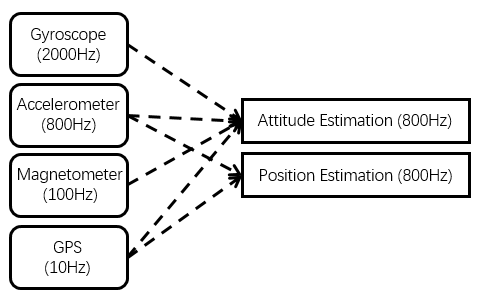
\includegraphics[width=0.7\textwidth]{state estimation.png}
	\bicaption{状态估计框架图}{Diagram of state estimation}
	\label{fig:stateestimation}
\end{figure} 

在本章中,我们将重点讨论系统中使用的状态估计方法(\autoref{fig:stateestimation})。我们将介绍由这些方法支持的系统飞行测试结果。我们注意到,自主飞行需要仔细地集成其他重要模块,如控制、校准等。这些模块的讨论放到后面两章。这些模块作为通用模块,以支持整个系统的运行。

\gdutsection{状态估计}{State estimation}
我们工作的核心是一个可靠的估计模块,该模块使用GPS、低成本的IMU和磁力计输出姿态、位置和速度。我们注意到,基于磁力计及GPS的偏航角估计较为特殊,因此,我们提出了一种解耦估计器设计。\par
我们将世界坐标系记为$\left\{ W \right\}$,将机体坐标系记为$\left\{ B \right\}$,将世界坐标系和机体坐标系中的向量分别定义为$(\cdot)^w$和$(\cdot)^b$。我们感兴趣的是世界坐标系中飞行器的姿态、位置和速度,其定义为
%\begin{equation}\label{eq:vector}
%\begin{bmatrix}
%	p^w_x & p^w_y & p^w_z & v^w_x & v^w_y & v^w_z & \phi^w & \theta^w & \psi^w
%\end{bmatrix}
%\end{equation}
$[p^w_x , p^w_y , p^w_z , v^w_x , v^w_y , v^w_z , \phi^w , \theta^w , \psi^w]$。
其中$p^w_x$、$p^w_y$和$p^w_z$是三维位置,$v^w_x$、$v^w_y$和$v^w_z$是三维速度,$\psi^w$、$\theta^w$和$\phi^w$是偏航角、俯仰角和横滚角,表示经过ZYX欧拉角转换后从机体坐标系到世界坐标系的旋转。因此,我们有旋转矩阵表示
\begin{equation}\label{eq:rotationmatrix}
	R_{b}^{w}=R(\psi^w)R(\theta^w)R(\phi^w)
\end{equation}\par
我们使用基于多传感器融合的状态估计方法来估计三维姿态、位置和速度。一种带延时观测的显式互补滤波器(ECF)将IMU数据与GPS融合,以提供横滚角($\phi^w$)和俯仰角($\theta^w$)的估计。解耦估计器将陀螺仪数据、磁力计数据和GPS融合,以提供偏航角($\psi^w$)的估计。一种带延时观测的三阶互补滤波器融合IMU和GPS数据输出三维位置和速度。

\gdutsubsection{横滚角、俯仰角估计}{Roll and pitch estimation}
直接安装在机体的惯性测量单元作为横滚角和俯仰角估计的主要信息来源。惯性测量单元(英文:Inertial measurement unit,简称IMU)是测量物体三轴姿态角(或角速率)以及加速度的装置。一般的,一个IMU内会装有三轴的陀螺仪和三个方向的加速度计,来测量物体在三维空间中的角速度和加速度,并以此解算出物体的姿态。\par
陀螺仪测量的是$\left\{ B \right\}$相对于$\left\{ W \right\}$的角速度,投影在机体系$\left\{ B \right\}$。
\begin{equation}\label{eq:gyromodel}
	\Omega^y=\Omega+b+\mu
\end{equation}
其中$\mu$表示加性测量噪声,$b$表示陀螺零偏。
姿态估计的第一步是将陀螺仪测量的角速度积分成陀螺仪的姿态。在早期的惯性导航应用中,因为计算机计算能力有限,人们曾经使用双速度积分法:高速一阶积分和中速高阶积分,从而在保证积分精度的前提下降低计算量\cite{savage1998strapdown}。在现在IMU的低精度应用中,一般单片机的计算性能足以保证在IMU的测量带宽内使用最精确的积分方法,因此我们没有必要讨论双速度积分法。在本文中,我们不考虑地球自身的旋转和地球的曲率,因此只限于小范围内的IMU的应用。陀螺仪积分出的姿态短时间内是准确的,但长时间后因为漂移误差精度会大幅下降\cite{钱华明2010基于}。\par
加速度计测量物体的比力,即去掉重力后的整体加速度或者单位质量上作用的非引力。
\begin{equation}\label{eq:accmodel}
	a=R^T(\dot{v}-g)+b_a+\mu_a
\end{equation}
其中$\mu_a$表示加性测量噪声,$b_a$表示加速度零偏,$\dot{v}$是世界系的加速度。
三轴加速度计的原理能够用来测量角度。在没有外力作用的情况下,加速度计能够精确地测量俯仰角和滚转角,且没有累积误差。由于加速度计本身的特性,加速度计解算的姿态很灵敏,非常容易受到振动以及运动加速度的影响\cite{赵翔2012基于}。

\gdutsubsection{偏航角估计}{Yaw estimation}
磁力计提供周围环境磁场的测量值。
\begin{equation}\label{eq:magmodel}
	m=R^T m^w+B_m+\mu_m
\end{equation}
其中$m^w$为在世界系的地球磁场矢量,$B_m$为局部磁场干扰,$\mu_m$为测量噪声。对于磁力计的读数,$\mu_m$通常是相当小的,但是,局部磁场干扰$B_m$可能是非常大的,特别是如果传感器被放置在电机的电源线附近。多旋翼飞行器通用的无刷电机在运转的时候就会产生变化的磁场,和地磁场叠加之后,通过这个有偏差的地磁向量作为参考去计算所得到的偏航角是不准确的,目前没有很好的办法去解决磁场干扰问题\cite{梅玲玉2019基于}。\par

\gdutsubsection{位置速度估计}{Position and velocity esitimation}
卫星导航系统(Global Navigation Satellite System, GNSS)是覆盖全球的自主地利空间定位的卫星系统,允许小巧的电子接收器确定它的所在位置(经度、纬度和高度),并且经由卫星广播沿着视线方向传送的时间信号精确到10米的范围内。在户外环境中,GPS通常用于提供位置、世界系的速度和航向角。GPS系统由一个24颗卫星组成的星座组成,这些卫星连续不断地围绕地球运行,高度为20180公里。GPS接收器的位置是通过观测卫星发送的信号的飞行时间来确定的,并被接收器探测到。如果接收机有准确的时间信息,则至少需要三个卫星信号来确定接收机的位置。然而,对于低成本的GPS接收器,也必须接收到定时信息,这需要至少4个卫星信号。存在各种各样的因素影响着GPS的估计。主要的误差来源包括卫星轨道数据不准确、卫星时钟不准确、信号通过电离层时的可变延迟、地球表面附近的天气状况以及来自附近建筑物和山脉的多径反射。GPS总体偏差约为5-10m。现代GPS接收机利用接收信号载波相位的多普勒频移来估计航向角和对地速度\cite{wendel2006integrated}。

\gdutsection{基于ECF的传感器融合}{ECF-based sensor fusion}
针对飞行器应用开发从业人员,我们希望设计一个模块化、容易扩展的传感器融合观测器。这意味着当我们需要增加或删除传感器时需要数学推导和编程的工作量应该是最小的。接下来我们将对目前流行算法的优缺点进行分析,以引出我们设计的融合框架。\par
一个标准的方法是使用扩展的随机线性估计技术\cite{lefferts1982kalman,barshan1995inertial}。另一种方法是使用确定性互补滤波器和非线性观测器设计技术\cite{zimmermann1992high,baerveldt1997low,vik2001nonlinear}。对于我们考虑的低成本、轻量化系统,线性滤波技术已被证明在应用场景中鲁棒性不强\cite{roberts2003low},而线性单输入单输出互补滤波器在实践中经常被使用\cite{saripalli2003tale,corke2004inertial}。前人关于非线性姿态观测者的研究有一个不足的地方是计算开销大,而且所构造姿态的误差较大。对于上述缺点,显式互补滤波器不需要对姿态进行在线代数重构。因此,该观测器非常适合在嵌入式硬件平台上实现。此外,对于不同的传感器数据的信任度可以在观测器响应中设置权重,这一特性允许开发人员根据传感器特定的噪声特性进行调整。最后,基于EKF的线性观测器方法在初始误差大时可能引起非常大的误差,而基于非线性控制方法的设计可以做到全局收敛。因此,我们采用基于ECF的非线性观测器的方法\cite{mahony2008nonlinear}。\par

\gdutsubsection{基于ECF的标准实现}{Standard implementation based on ECF}
姿态估计的目标是为估计量$\hat{R}(t)\in SO(3)$提供一组动力学方程来使得误差旋转矩阵$\widetilde{R}(t)\rightarrow I_3$。飞行器的姿态运动学方程为
\begin{equation}\label{eq:kinematics}
	\dot{R}=R\Omega_{\times}=(R\Omega)_{\times}R
\end{equation}
其中,$\Omega$是机体角速度。作者所提出的观测器方程直接作为一个运动学系统用于姿态估计。此观测器运动学包括基于测量的预测项和由误差导出的修正项。记$\hat{R}$表示对飞行器姿态$R$的估计。观测器的一般形式是
\begin{equation}\label{eq:passivefilter}
	\dot{\hat{R}}=\hat{R}(\Omega_{\times}+k_P \mathbb{P}_a(\widetilde{R}))
\end{equation}
其中,$k_P>0$。观测器框架如\autoref{fig:DiagramECF}所示。
\begin{figure}[htbp]
	\centering
	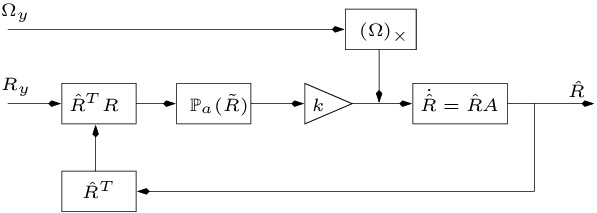
\includegraphics[width=0.7\textwidth]{Block-diagram-of-the-simplified-form-of-the-passive-complementary-filter.png}
	\bicaption{显式互补滤波框架图}{Block diagram of explicit complementary filter}
	\label{fig:DiagramECF}
\end{figure}
对于$\mathbb{P}_a(\widetilde{R})$,我们可以使用欧拉角相减,DCM或四元数相乘来获取姿态的误差,这样的方法都有一个缺点,那就是需要通过加速度计和磁力计的测量计算出一组姿态。虽然常用的方法比较成熟,但也有一些问题,比如欧拉角法存在奇异点(如在俯仰角90度时),DCM和四元数的TRIAD或QUEST等方法又需要额外的计算。ECF的突出贡献之一就是直接利用加速度计和磁力计的测量值,利用和惯性空间向量的叉乘,简单地就获得了姿态的误差。如下观测器是ECF的标准形式
\begin{equation}\label{eq:Explicitfilter}
	\begin{aligned}
	\dot{\hat{R}}&=\hat{R}((\Omega^y - \hat{b})_{\times}+k_P (\omega_{mes})_{\times})\\
	\dot{\hat{b}}&=-k_I \omega_{mes}\\
	\omega_{mes} &\coloneqq \sum_{n=1}^{n} k_i v_i \times \hat{v}_i	
	\end{aligned}
\end{equation}
其中$k_P$,$k_I$,$k_i$是任意非负的观测器增益。注意到姿态$\hat{R}$是整个观测器的输出。在文献\cite{mahony2008nonlinear}中对观测器(\autoref{eq:Explicitfilter})进行了广泛的研究,表明姿态和零偏能做到指数收敛(理论和实验)。该滤波器具有互补的特性,利用陀螺仪信号的高频部分和磁力计、加速度计的低频部分\cite{mahony2008nonlinear}。与这些信号相关联的截止频率由增益$k_P$,$k_I$,$k_i$决定。\par
用于表示旋转的单位四元数在代码实现中具有较高的效率,是实现$SO(3)$群运算的常用方法。上述观测器的四元数表示如下
\begin{equation}\label{eq:quatfilter}
	\begin{aligned}
	\dot{\hat{q}}&=\frac{1}{2} \hat{q} \otimes \mathbf{p}(\Omega_y - \hat{b} + k_P \omega_{mes})\\
	\dot{\hat{b}}&=-k_I \omega_{mes}\\
	\omega_{mes} &\coloneqq \sum_{n=1}^{n} k_i v_i \times \hat{v}_i	
\end{aligned}
\end{equation}\par
如果飞行器配备了GPS系统,估计速度和位置是一个简单的过程。在这种情况下,位置运动学是线性的,可以使用线性滤波器。记$\hat{p}$表示位置的估计,$\hat{v}$表示速度的估计。给出了一个简单的线性滤波器
\begin{equation}\label{eq:posfilter}
	\begin{aligned}
		\dot{\hat{p}}&=\hat{v}-k_x (\hat{p}-p_{GPS})\\
		\dot{\hat{v}}&=\hat{R}^T a - g e_3 - k_v (\hat{p}-p_{GPS})\\	
	\end{aligned}
\end{equation}
其中增益$k_x,k_v > 0$。只要姿态估计是准确的,这个滤波器具有很强的鲁棒性。此观测器可以很容易地加上加速度计的零偏估计。并且可以使用卡尔曼滤波去调节$k_x$和$k_v$。在实际应用中,对于微型飞行器系统,测量的噪声特性非常差,因此通常最好使用恒定增益滤波器,而不是引入附加的复杂性和潜在的不稳定性的Riccati方程与卡尔曼滤波器。

\gdutsubsection{使用gps辅助的姿态观测器设计}{GPS-aided attitude observers}
大多数现有的姿态观察器/滤波器都依赖于小加速度假设($\dot{v}\approx 0$),因此重力方向测量可以近似于上一小节中讨论的加速度计测量。然而,对于许多飞行器都有高速运动的场景,会产生比较大的线性加速度,姿态估计器的输出可能会有较大的误差。对于较大的线性加速度,可以将GPS线速度的补充测量与加速度计的测量相结合来估计飞行器的加速度,从而提高姿态估计的精度。基于ECF的使用GPS辅助的姿态观测器被提出\cite{hua2010attitude}。值得注意的是,文中提出的观测器不能保证从磁场测量中对横滚角和俯仰角估计的解耦。\par
我们使用直接补偿的方法。只要与飞行器惯性运动相关的加速度分量得到补偿,加速度计的数据也可以使用。最简单的方法是使用绝对测量信号GPS来估计飞行器的加速度
\begin{equation}
	a_{CTD}=a_{IMU}-\hat{R}^T \dot{v}_{GPS}
\end{equation}
其中$a_{CTD}$是修正后的加速度。在这种情况下,满足$a_{CTD} \approx R^T e_3$,$a_{CTD}$能提供准确的姿态信息。值得注意的是,在上文提出的互补滤波器中,只需要$a_{CTD}$的低频成分。因此,GPS速度的一阶导数$\dot{v}_{GPS}$中的噪声影响较小。

\gdutsubsection{处理耦合问题}{Handling coupling issues}
在补偿了运动加速度后,使得假设$a_{CTD} \approx R^T e_3$成立,在这种情况下我们依然可以使用显式互补滤波器的标准实现(\autoref{eq:Explicitfilter}),我们这里再将修正项单独拿出来讨论
\begin{equation}
\omega_{mes} \coloneqq k_1 u_B \times \hat{u}_B + k_2 m_B \times \hat{m}_B	
\end{equation}
其中,增益$k_{1,2}>0$,$u_B = a_B / g$,$u_I = e_3$,$\hat{u}_B = \hat{R}^T u_I$,$\overline{m}_B = m_B / \left| m_I \right|$,$\overline{m}_I = m_I / \left| m_I \right|$,$\hat{\overline{m}}_B = \hat{R}^T \overline{m}_I$。然而,研究人员已经认识到这个标准实现存在一些耦合问题,这些问题在文献\cite{hua2013implementation,hua2011nonlinear,martin2007invariant}中已经进行了深入的讨论。\par
磁场干扰和零偏会影响横滚角和俯仰角的估计。在实际应用中,特别是在使用电机作为执行器的小型飞行器中,较大的磁场干扰几乎是不可避免的,导致$m_B$和$R^T m_I$之间存在较大的时变误差。这不仅会导致偏航角的估计误差很大,而且还会导致横滚角和俯仰角估计产生误差。
滚转角,俯仰角和偏航角估计的动力学方程是高度耦合的。这意味着偏航角的估计会较大地影响着横滚角和俯仰角的估计。在实际应用中,重力矢量和地球磁场矢量(即$e_3$和$m_I$)可能是“无法使用的”,因为两个向量在某些地区是非常接近的。在这种情况下,$\overline{m}_I$的z轴分量比x、y轴分量大很多。在高纬度地区,如法国$\overline{m}_{I,3}\approx 0.9$。因此,横滚角和俯仰角的动力学与偏航误差动力学是紧耦合的。另一方面,使用两个非常接近的向量$e_3$和$\overline{m}_I$也可能导致不可能构造出完整的姿态信息。
很多文献考虑了对输入信号的解耦,以确保横滚角和俯仰角估计不受磁场干扰的影响,对显式互补滤波器标准实现进行修改,以提高姿态估计的整体质量。让我们讨论一下这些策略。\par
解耦的关键在于能否在计算上区分开来,由于我们将磁场向量转换到机体系上做修正,并且磁场向量本身包括x轴,y轴分量,这些分量会影响到roll、pitch分量。我们完全可以将roll、pitch分量的四元数和偏航分量的四元数分离开,当我们获取到磁力计数据时,我们只用磁力计修正偏航分量的四元数,然后生成一个完整的姿态。\par
注意到在姿态修正过程中roll、pitch分量和yaw分量的明显区别,我们首先将姿态划分为roll、pitch分量四元数和yaw分量四元数:
\[
q^{RP} = 
\begin{bmatrix}
	q_w^{RP} \\
	q_x^{RP} \\
	q_y^{RP} \\
	q_z^{RP}
\end{bmatrix},
\hspace{1em}
q^{Y} = 
\begin{bmatrix}
	q_w^{Y} \\
	q_x^{Y} \\
	q_y^{Y} \\
	q_z^{Y}
\end{bmatrix}
\]。
我们通过对姿态四元数分解,其关系为:
\begin{equation}\label{eq:decompose}
	q = q^{Y} \otimes q^{RP}	
\end{equation}
由此我们可以看出,对完整的姿态四元数修正实际上是不必要的,偏航分量只对应于$q^{Y}$。我们可以通过磁力计/GPS计算的偏航角只修正$q^{Y}$,然后通过\autoref{eq:decompose}叠加到完整的姿态四元数上。由于roll、pitch分量只存在于四元数$q^{RP}$,因此避免了磁场干扰对roll、pitch的影响。由于欧拉角定义的旋转顺序是ZYX,偏航分量四元数可以写成:
\begin{equation}
	q^{Y} = 
	\begin{bmatrix}
		cos(\frac{\hat{\psi}}{2}) \\
		0 \\
		0 \\
		sin(\frac{\hat{\psi}}{2})
	\end{bmatrix}	
\end{equation}
偏航修正方式可以按照线性互补的方法进行修正:
\begin{equation}
	\hat{\psi} = k_Y (\psi_{mag} - \hat{\psi}) 	
\end{equation}
\gdutsection{实验结果}{Experimental results}
本章给出了两个实验:(1)与信号良好的GPS/RTK的位置、速度及差分的加速度比较,研究了估计器的性能;(2)飞行器的飞行实验;第1章讨论了实验平台的结构。第四章将介绍控制方法。

\gdutsubsection{评估估计器的性能}{Evaluating estimator performance}
我们希望通过与真值对比以研究估计器的性能,真值是由厘米级精确度的GPS/RTK系统定义的。本小节的实验分为两部分。第一部分为飞行器飞行时,通过比较板载估计器输出与的GPS/RTK来评估估计的准确性。在本次实验中,估计器能很好地跟上GPS/RTK输出的真值。第二部分考察了使用来自估计器的姿态和速度反馈来维持姿态、速度和位置的反馈控制。

\gdutsubsection{飞行器飞行实验}{UAV flying test}

\gdutsection{总结与讨论}{Summary and discussion}
在本章中,我们展示了使用IMU作为主要传感器,融合其他传感器进行状态估计以实现飞行器的稳定飞行。关键技术是考虑了传感器延时,运动加速度补偿以及异常处理相关的算法。此外,我们将容易受到磁场干扰的偏航角和俯仰、横滚角解耦以保证系统的鲁棒性。本文提出的算法可以使飞行器保持稳定。

\gdutchapter{传感器校准}{Sensor calibration}
在本章中,我们研究如何使用较少的仪器来进行高精度的传感器校准以提供更好的传感器数据。一般来说,基于MEMS的传感器的精度都比较差,远远达不到高精度导航的要求。然而,开发基于MEMS的传感器的飞行器,要保证传感器数据精度是很困难的。在本章中,我们研究传感器校准算法,开发了一种不需要外部设备就可以进行较高精度的校准。我们详细介绍了基于优化的传感器校准算法,并将其与融合和控制方法(第4章)结合起来进行实验,以验证系统的性能。\par
本系统的关键技术是一种传感器校准算法,能够无需外部设备的情况下进行校准。我们要求校准算法能够使用人手就能完成,无需外部设备,在尽量简单的校准流程下保证校准结果的准确性。\par

\gdutsection{加速度计校准}{Acceleromter calibration}
首先建立加速度计的传感器模型,并利用重力的向量大小进行标定\cite{jekeli2012inertial}。对于加速度计,我们使用静态检测的方法\cite{fong2008methods},并使用基于方差的检测算法\cite{sabatini2006wavelet}。由于需要提取静止的重力向量,我们可以对原始数据进行静态检测,放宽校准种严格的静止的条件。利用校准后的参数将原始数据转化为标准的重力向量$g$。\par
我们的检测器基于基于Tedaldi的方法:对于每个加速度计样本$\begin{bmatrix}
	a^t_x & a^t_y & a^t_z
\end{bmatrix}$,给定一个长度为t秒的时间间隔时刻,我们计算方差的大小
\begin{equation}\label{eq:var}
	\zeta(t)=\sqrt{[var_{t_w}(a^t_x)]^2+[var_{t_w}(a^t_y)]^2+[var_{t_w}(a^t_z)]^2}
\end{equation}
其中$var_{t_w}(a^t)$是一个运算符,计算加速度计$a^t$在以$t$为中心,长度为$t_w$秒的时间间隔内的方差。我们通过判断$\zeta(t)$是否小于或大于一个阈值对静态和运动间隔进行分割。与传统的六面校准法相比\cite{尹杭2014一种},该方法在可以在任意姿态下保持静止。

\gdutsubsection{传感器误差模型}{Sensor error model}
对于加速度计,有
\begin{equation}\label{eq:axiserror}
	T^{a}=
	\begin{bmatrix}
		1 & \beta_{yz} & \beta_{zy}\\
		\beta_{xz} & 1 & \beta_{zx}\\
		\beta_{xy} & \beta_{yx} & 1
	\end{bmatrix}
\end{equation}
其中,$T^a$是轴正交矩阵,$\beta_{ij}$是第$i$个传感器轴的误差对第$j$个轴的造成的误差影响。\par
此外,加速度计受到零偏和尺度误差的影响。引入尺度矩阵
\begin{equation}\label{eq:scaleerror}
	K^{a}=
	\begin{bmatrix}
		s^a_x & 0 & 0\\
		0 & s^a_y & 0\\
		0 & 0 & s^a_z
	\end{bmatrix}
\end{equation}
我们接着引入零偏向量
\begin{equation}\label{eq:scaleerror}
	b^{a}=
	\begin{bmatrix}
		b^a_x\\
		b^a_y\\
		b^a_z
	\end{bmatrix}
\end{equation}
完整的传感器误差模型为
\begin{equation}\label{eq:sensorerrormodel}
	a^O=T^a K^a (a^S + b^a + \nu^a)
\end{equation}
其中,$a^O$和$a^S$分别表示校准后和校准前的加速度数据,$ν^a$是加速度计测量噪声。

\gdutsection{陀螺仪校准}{Gyroscope calibration}
一般来说,对于陀螺仪校准,要完整校准出零偏、尺度和轴正交要比加速度计校准复杂得多。即使对角速度精度有较高得要求,由于缺乏相应的设备,也无法校准出陀螺仪的尺度和轴正交参数。简单的陀螺校准无法用于高精度的导航上。因此,基于Tedaldi的方法\cite{tedaldi2014robust},我们将对陀螺仪进行十二参数的标定。

\gdutsection{磁力计校准}{Magnetometer calibration}
磁力计本身的系统误差非常大,直接用原始数据计算偏航角的精度十分差以至于无法用于控制飞行器的偏航。因此,我们基于椭球拟合的方法来校准磁力计\cite{李勇2012基于椭球拟合的三轴磁传感器误差补偿方法}。我们使用牛顿迭代法求解最小二乘问题,因为代价函数是非线性的。传感器测量模型与章节3.1相同。

\gdutsection{实验结果}{Experimental results}
实验环境不需要任何外部设备。在所有的实验中,我们只需要采集传感器的原始数据。实验平台在第1章中进行了讨论。实验平台是基于开源飞控。这个现成的飞控板配有一个IMU、一个磁力计和一个STM32微控制器。

\gdutsubsection{加速度计校准结果}{Accelrometer calibration result}
在本实验中,采集IMU原始数据,使其以任意姿态静止。整个校准流程为3分钟。校准精度是根据重力模长进行评估的。加速度计校准结果显示在。

\gdutsubsection{陀螺仪校准结果}{Gyroscope calibration result}
这个实验给出陀螺校准结果。陀螺仪和加速度计同时校准。校准精度是根据角度误差来评估的。陀螺仪校准结果显示在。

\gdutsubsection{磁力计校准结果}{Magnetometer calibration result}
在本实验中,采集磁力计原始数据,以足够多的姿态运动飞控。校准精度根据磁场模长进行评估。磁力计校准结果显示在。

\gdutsection{总结与讨论}{Summary and discussion}
在本章中,我们提出了一种IMU校准算法,该方法能够在无需外部设备的情况下进行校准。我们对校准评估标准方法的进行优化。我们的方法能够使精度提高到xxx。

\gdutchapter{控制}{Control methods}
本章讨论如何调整控制方法,以配合飞行器稳定飞行的需要。我们介绍了保证状态估计和控制平滑的系统体系结构。

\gdutsection{反馈控制}{Feedback control}
在给定估计的状态后,我们让飞行器用位置跟踪控制器来跟踪所需的轨迹\cite{lee2010geometric}。由传感器融合模块(第二章)的状态估计直接作为控制器的反馈。在本文的设计中,姿态控制器和位置控制器都在STM32以400Hz的频率运行。

\gdutsection{实验结果}{Experimental results}
我们有一个基于多传感器融合的状态估计器来产生800Hz的位置、速度、姿态估计,足以稳定飞行器。\par
在这个实验中,飞行器以大约1米/秒的速度自动沿着矩形轨迹生成平滑轨迹。使用GPS/RTK在信号良好的状态下来量化全局跟踪性能。由图xxx可以看出,飞行器的实际位置收敛到期望位置,其标准差为xxx,表明控制器的稳定收敛。

\gdutbackmatter
\gdutchapter{结论与展望}{Conclusion and prospect}
在这篇论文中,我们展示了对飞行器自主飞行的最新技术的贡献,大部分贡献是状态估计算法。在第三章中,我们开发了状态估计系统,提出了一种模块化和可扩展的方法,该方法能够以一致的方式组合来自多个传感器的信息。在第四章中,我们开发了传感器校准算法,能够在没有外部设备的情况下对传感器进行高精度的校准。在第五章中,我们提出的控制方法结合前两章的算法形成一个集成的飞行器系统。\par
我们注意到,虽然主要的实验平台使用的是四旋翼,但我们的方法不限于这一特定类型的平台。实际上,我们的方法是基于传感器的,同样适用于其他机器人,如固定翼、地面机器人等。
\gdutbacksection{成果总结}
综上所述,本文的主要贡献如下:
\begin{itemize}
	\item 我们开发了算法和系统,使计算资源受限的飞行器能够自主飞行,只使用低成本的传感器。
	\item 我们提出了一种算法,通过互补融合来自多传感器的信息来提高系统的可靠性。
	\item 我们提出了一种算法,无需外部设备就能够进行传感器校准。
	\item 我们开发集成了控制算法,并通过大量的实验表明,飞行控制系统是稳定可靠的。
\end{itemize}

\gdutbacksection{未来研究展望}
本文涉及到了几个有趣的研究领域,其中一些是随着飞行器技术的发展而不断发展成大型系统的,而另一些则是我们在评估最新方法的性能时值得追求的新方向。
\paragraph{自主飞行中估计与控制的耦合设计。}
在我们目前的工作中,控制器与估计器是分开设计的。然而,随着我们朝着高速自主飞行的方向发展,我们可能会要求估计器和控制器耦合设计,以生成和执行高效、无碰撞和安全的飞行轨迹。
\paragraph{用于飞行器的新的传感器技术。}
虽然传统的传感器如IMU、GPS、相机已被证明可用于飞行器导航,但最近传感技术的发展可能创造新的机会。例如,光场可以作为深度感知的传感器。这些新型传感技术在飞行器上的应用具有很大的潜力。
\paragraph{传感器和能观性研究。}
众所周知,传感器数量越多,系统的能观性越好,但单个传感器对系统能观性的影响尚不清楚。增加更多的传感器会带来出更多的能观性,但是传感器提供的信息以及信息的质量会导致能观性的复杂判断条件。因此,一个能够以在线方式识别能观性的通用框架将有利于更高层次的任务,如运动规划和风险评估。

\nocite{*}% 列出全部参考文献
\printbibliography

\gdutchapter{攻读学位期间取得与学位论文相关的成果}{Publication and patents during study}

\gdutbacksection{发表和投稿与学位论文相关学术论文}

\begin{results}
  \item \textbf{张三}, 李四, 等. Jet electrochemical machining of micro dimples with conductive mask.
  Journal of Materials Processing Technology. 2018, 257:101-111. (SCI Impact Factor 3.647,
  WOS:000431161400010)
  \item 李四, \textbf{张三}, 王五, 等. Electrochemical direct-writing machining of micro- channel array.
  Journal of Materials Processing Technology. 2019, 265:138-149. (SCI Impact Factor 3.647,
  WOS:000451935100014)
\end{results}

\gdutbacksection{申请发明专利}

\begin{results}
  \item 李四, \textbf{张三}, 王五. 一种微流道电解加工装置. 发明专利申请号: 201810467763.5.
\end{results}

\gdutstatement

\gdutchapter{致谢}{Acknowlegements}
\zhlipsum[1]

\gdutappendix

\gdutchapter{附录标题}{The appendix title}
对需要收录于学位论文中且又不适合书写于正文中的附加数据、资料、详细
公式推导、计算机程序等有特色的内容,可做为附录排写。
\end{document}